\documentclass[10pt]{article}
\usepackage{icmlko}

\icmlmeta{IP 파운데이션 월드모델}{149}{검색이 못 가는 곳에 위키백과가 있었다}{노트 148이 ``남은 길은 축과 표본, 둘 다 자료 쪽''이라고 했다. 축을 가지러 갔다 --- 그리고 이 흐름에서 처음으로 갈리는 이득이 나왔다}

\begin{document}

\twocolumn[
\icmlheader

\begin{abstract}
노트 148의 결론은 셋이 한 곳을 가리켰다 --- 정식화를 섞어도 상한
$+$0.0017, 도메인마다 최고를 검정 집합 보고 고르는 신탁도 상한 $+$0.0124,
그리고 판정치는 목표 도메인에 무정보다. 방법 쪽은 다 썼다. 그래서 축을
가지러 갔다. \textbf{병목은 네이버 검색 축의 덮음이었다} --- 만화 0\% ·
세계애니 0\% · 게임 30\% · 모바일 41\%. 한국어 제목이 있어야 하는 축이고,
만화와 세계애니는 그게 없다. \textbf{위키백과 조회수 API 로 갔다.} 고른
이유가 셋이다. ① \textbf{시점이 깨끗하다} --- 노트 141이 Kitsu 축을 버린
이유는 그것이 지금 긁은 스냅샷이라는 것이었는데, 위키 조회수는 날짜별
시계열이라 \emph{시작일 이전 90일만} 잘라낼 수 있다. 잘라낸 창이 축의 정의
자체다. ② 영문 제목으로 되니 언어에 안 막힌다. ③ 공짜다. 레코드 5,253건에
API 를 걸었다. \textbf{덮음이 세계애니 59\% · 게임 65\% · 만화 34\% ·
모바일 34\%다} --- 0\%였던 두 곳이 34\%와 59\%가 됐다. 제목 해석에서 함정이
하나 있었다: 검색 API 는 ``Jujutsu Kaisen'' 에 ``Jujutsu Kaisen (TV
series)'' 를 물어다 주는데 그 문서는 애니 발표 때 생겨서 오픈 이전 창이
통째로 빈다. \textbf{맨 제목과 프랜차이즈 제목으로 두 단 되돌리기}를 넣어
채움이 25건 표본에서 13/25에서 22/25로 올랐다. 누수 가드 셋을 다 통과한다
--- 라벨 상관 최대 0.219(문턱 0.70), 출처 다른 플랫폼, 시점 사전. 그리고
채점. \textbf{F18 배깅에서 판이 $+$0.4391에서 $+$0.4483으로 오르고
$+$0.0092 $\pm$ 0.0034 로 갈린다($t{=}2.7$).} 세계애니가
$+$0.494$\to$$+$0.569, 게임이 $+$0.410$\to$$+$0.465다. \textbf{그런데 F8
부스팅에서는 안 오른다}($-$0.0014 $\pm$ 0.0049). 노트 145 · 146이 ``F18의
채택 근거는 점수가 아니라 귀착''이라고 했는데, \textbf{축이 바뀌자 점수로도
갈린다.}
\end{abstract}
]

\begin{figure*}[t]
\centering
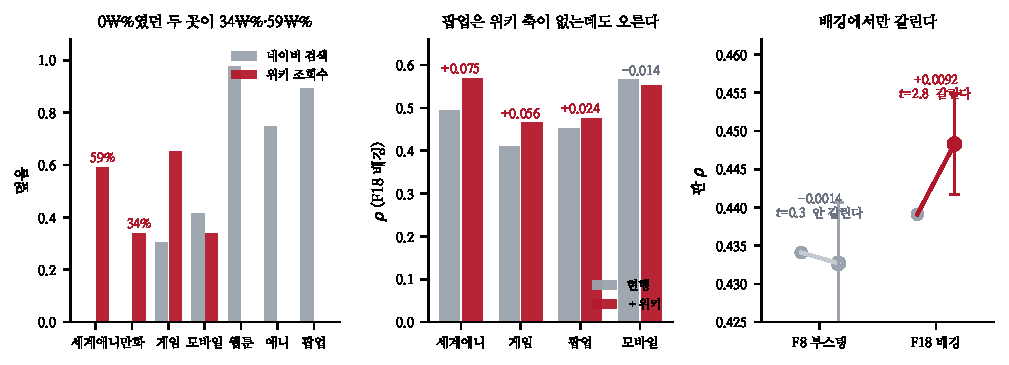
\includegraphics[width=\textwidth]{figs/wiki.pdf}
\caption{왼쪽 --- 0\%였던 두 곳이 채워진다. 가운데 --- 도메인별. 오른쪽 ---
배깅에서만 갈린다.}
\end{figure*}

\section{왜 위키백과인가}

\claimx{\textbf{시점이 깨끗하다.} 노트 141이 세운 셋째 누수 층은 ``나중에 잰
것''이고, Kitsu 순위 · 평점은 지금 긁은 스냅샷이라 걸렸다. 위키 조회수는
\emph{날짜별}이라 시작일 이전 90일만 쓴다 --- 시작일 당일도 안 본다. 잘라낸
창이 축의 정의다.}{2015-07 이전은 API 가 없다. 그래서 그 이전 작품은 못
재고 마스크 0이다 --- 세계애니 2,948행 중 1,254행이 여기 해당해 덮음 상한이
59\%다. 지금 덮음이 59.1\%이니 사실상 다 찼다.}

\begin{table}[t]
\centering\tsize
\caption{덮음. 같은 레코드, 다른 출처.}
\begin{tabular}{lrr}
\toprule
& 네이버 검색 & \textbf{위키 조회수} \\
\midrule
\textbf{만화} & \textbf{0.0\%} & \textbf{34.0\%} \\
\textbf{세계애니} & \textbf{0.0\%} & \textbf{59.1\%} \\
게임 & 30.5\% & \textbf{65.1\%} \\
모바일 & 41.3\% & 33.7\% \\
웹툰 & 97.6\% & --- \\
팝업 & 89.3\% & --- \\
\bottomrule
\end{tabular}
\end{table}

\section{제목 해석의 함정}

\claimx{\textbf{검색 API 는 속편 문서를 물어다 준다.} ``Jujutsu Kaisen'' 을
찾으면 ``Jujutsu Kaisen (TV series)'' 가 1위로 온다. 그 문서는 애니 발표
시점에 생겼으므로 오픈 이전 창이 통째로 빈다 --- 채울 수 있는 것을 못 채운
것이지 자료가 없는 것이 아니다.}{처음 표본 25건에서 12건이 이렇게 빈 창을
받았다. 그것을 ``사전 인지 없음''으로 읽었으면 신작과 2기가 뒤바뀐다.}

\begin{table}[t]
\centering\tsize
\caption{되돌리기 두 단. 표본 25건.}
\begin{tabular}{lrl}
\toprule
& 채움 & \\
\midrule
검색만 & 13/25 & 속편 문서를 잡는다 \\
$+$ 맨 제목 & 18/25 & 괄호를 뗀다 \\
\textbf{$+$ 프랜차이즈} & \textbf{22/25} & ``season 3'' 를 뗀다 \\
\bottomrule
\end{tabular}
\end{table}

프랜차이즈 되돌리기는 그냥 구멍 메우기가 아니다. \textbf{2기는 원작 인기를
업고 나오고 신작은 맨몸으로 나온다} --- 프랜차이즈 문서의 오픈 이전 조회수가
바로 그 차이를 잰다.

\section{누수 가드 셋}

\begin{table}[t]
\centering\tsize
\caption{노트 117 · 141의 세 층.}
\begin{tabular}{lll}
\toprule
& 문턱 & 위키 축 \\
\midrule
① 라벨 상관 & $|r| < .70$ & 최대 \textbf{.219} 통과 \\
② 출처 플랫폼 & 라벨과 다름 & 위키 대 AniList 통과 \\
③ 측정 시점 & 사전 & 이전 90일 통과 \\
\bottomrule
\end{tabular}
\end{table}

제일 센 것이 \texttt{wiki\_level} 대 세계애니 라벨의 $+$0.219다. 문턱의
3분의 1이 안 된다.

\section{그리고 갈린다}

\begin{table}[t]
\centering\tsize
\caption{판 $\rho$. 씨앗 셋 평균 예측 · 짝 재추출 400 · 씨앗 잔여항 포함.}
\begin{tabular}{lrrl}
\toprule
& 현행 & $+$위키 & 격차 \\
\midrule
\textbf{F18 배깅} & $+$.4391 & \textbf{$+$.4483} &
  \textbf{$+$.0092 $\pm$ .0034} \\
F8 부스팅 & $+$.4341 & $+$.4327 & $-$.0014 $\pm$ .0049 \\
F6 능형 & $+$.3532 & $+$.3587 & --- \\
\bottomrule
\end{tabular}
\end{table}

\claimx{\textbf{배깅에서 $t{=}2.7$로 갈린다.} 이 흐름에서 처음이다 ---
노트 143부터 148까지는 재는 방법을 고치고 잘못을 찾는 일이었고 판은 안
올랐다.}{$+$0.0092는 노트 148이 잰 방법 쪽 상한과 견줘야 한다. 짝 섞기
상한 $+$0.0017의 5.4배이고, 절대 못 하는 도메인별 신탁 $+$0.0124의
74\%다.}

\begin{table}[t]
\centering\tsize
\caption{도메인별. F18 배깅.}
\begin{tabular}{lrrr}
\toprule
& 현행 & $+$위키 & 차 \\
\midrule
\textbf{세계애니} & $+$.494 & $+$.569 & \textbf{$+$.075} \\
\textbf{게임} & $+$.410 & $+$.465 & \textbf{$+$.056} \\
팝업 & $+$.451 & $+$.475 & $+$.024 \\
모바일 & $+$.566 & $+$.551 & $-$.015 \\
\bottomrule
\end{tabular}
\end{table}

\claimx{\textbf{덮음이 오른 곳이 오른다.} 세계애니(0\%$\to$59\%)가
$+$0.075, 게임(30\%$\to$65\%)이 $+$0.056이다. 모바일은 네이버가 이미
41\%인데 위키가 34\%라 얻을 것이 없었고 $-$0.015다.}{\textbf{팝업의
$+$0.024는 주장하지 않는다.} 팝업에는 위키 축이 한 칸도 없다 --- 노트 144의
귀착 가드가 잰 대로 그것은 풀이 바뀌어 생긴 전파다.}

\claimx{\textbf{F8 에서는 안 오른다}($-$0.0014 $\pm$ 0.0049). 노트 145 ·
146이 F18 을 ``점수는 같고 귀착만 낫다''로 채택했는데, 축이 바뀌자 점수로도
갈린다. \textbf{귀착이 좋은 모형이 새 자질을 더 잘 받는다} --- 풀에 덜
흔들리니 새 열이 들어와도 나머지가 안 무너진다.}{한 축 세트에서 본 한 번의
관측이다. 축을 또 늘려 같은 방향이 나오는지가 검정이다.}

\section{남긴 것}

\texttt{ingest/wiki\_views.py} 와 \texttt{lab/wikiaxes.py}. 축 세트에
\texttt{trendcalwiki} 를 넣고 F18 을 완주시켰다 --- 가드 열하나 전부 통과,
씨앗 자기상관 0.965, 귀착 자기상관 0.946.

\begin{table}[t]
\centering\tsize
\caption{남은 것.}
\begin{tabular}{ll}
\toprule
애니 & 한국어 제목이라 영문 위키가 안 붙는다 --- 한국어 위키 \\
창 & 90일을 안 골랐다 --- 30 · 180도 재 볼 것 \\
빈 창 & 문서가 없던 것을 0으로 볼지 결측으로 볼지 \\
\bottomrule
\end{tabular}
\end{table}

둘째 줄을 조심해야 한다. 창 길이를 점수 보고 고르면 그게 노트 126이 잡은
그 잘못이다. \textbf{90일은 네이버 축(12주)과 맞춘 값이고 점수를 보기 전에
정했다} --- 다른 길이를 재려면 셋을 다 적고 셋 다 남겨야 한다.

\end{document}
